\section{Auswertung}
\label{sec:Auswertung}

\subsection{Wheatston'sche Brückeschaltung}
Mit Hilfe der Wheatston'schen Brückeschaltung werden zwei unbekannte Wiederstände $R_{13}$ = Wert13 und $R_{14}$ = Wert14 bestimmt. Dies geschieht mit Formel ??, die Werte und Ergebnisse sind in den Tabellen \ref{tab:Wheat1} und \ref{tab:Wheat2} aufgeführt. $\overline{R_\text{13,14}}$ entspricht hierbei den gemittelten Werten für die gesuchten Widerstände.
\begin{table}[H]
  \centering
  \begin{tabular}{c c c c c}
    \toprule
    $R_2$ / $\Omega$ & $R_3$ / $\Omega$ & $R_4$ / $\Omega$ & $R_{13}$ / $\Omega$ & $\overline{R_{13}}$ / $\Omega$ \\
    \midrule
    332 & 735 & 265 & \num{322.8 +- 1.6} &  \\
    500 & 648 & 352 & \num{321.0 +- 1.6} &  \num{326.6 +- 0.9}\\
    664 & 582 & 418 & \num{336.0 +- 1.7} &  \\
  \end{tabular}
  \caption{Werte für die Bestimmung von $R_{13}$.}
  \label{tab:Wheat1}
\end{table}

\begin{table}[H]
  \centering
  \begin{tabular}{c c c c c}
    \toprule
    $R_2$ / $\Omega$ & $R_3$ / $\Omega$ & $R_4$ / $\Omega$ & $R_{14}$ / $\Omega$ & $\overline{R_{14}}$ / $\Omega$ \\
    \midrule
    332 & 493 & 507 & \num{920.8 +- 4.6} &  \\
    500 & 391 & 609 & \num{920.5 +- 4.6} &  \num{921.9 +- 2.7}\\
    664 & 336 & 664 & \num{924.5 +- 4.6} &  \\
  \end{tabular}
  \caption{Werte für die Bestimmung von $R_{14}$.}
  \label{tab:Wheat2}
\end{table}

\subsection{Kapazitätsmessbrücke}
Mit Hilfe der Kapazitätsmessbrücke werden drei unbekannte Kapazitäten $C_2$ = Wert2, $C_3$ = Wert3 und $C_8$ = Wert8 bestimmt. Dies geschieht mit Formel ??, die Werte und Ergebnisse sind in den Tabellen \ref{tab:Kapa1} bis \ref{tab:Kapa3} aufgeführt. $\overline{C_\text{2,3,8}}$ entspricht hierbei den gemittelten Werten für die gesuchten Kapazitäten.
\begin{table}[H]
  \centering
  \begin{tabular}{c c c c c}
    \toprule
    $C_2$ / nF & $R_3$ / $\Omega$ & $R_4$ / $\Omega$ & $C_2$ / 10$^{-6}$ \cdot F & $\overline{C_2}$ / 10$^{-6}$ \cdot F \\
    \midrule
    597 & 285 & 715 & \num{1.498 +- 0.007} &  \\
    750 & 329 & 671 & \num{1.530 +- 0.008} &  \num{1.517 +- 0.004}  \\
    994 & 395 & 605 & \num{1.522 +- 0.008} &  \\
  \end{tabular}
  \caption{Werte für die Bestimmung von $C_2$.}
  \label{tab:Kapa1}
\end{table}

\begin{table}[H]
  \centering
  \begin{tabular}{c c c c c}
    \toprule
    $C_2$ / nF & $R_3$ / $\Omega$ & $R_4$ / $\Omega$ & $C_3$ / 10$^{-6}$ \cdot F & $\overline{C_3}$ / 10$^{-6}$ \cdot F \\
    \midrule
    597 & 593 & 607 & \num{4.091 +- 0.020} &  \\
    750 & 639 & 361 & \num{4.237 +- 0.021} &  \num{4.165 +- 0.012}  \\
    994 & 705 & 295 & \num{4.159 +- 0.021} &  \\
  \end{tabular}
  \caption{Werte für die Bestimmung von $C_3$.}
  \label{tab:Kapa2}
\end{table}



\begin{table}[H]
  \centering
  \begin{tabular}{c c}
    \toprule
    f / Hz & $U_\text{br}$ / V \\
    \midrule
      20	  &  2.28  \\
      70	  &  1.88  \\
      180	  &  0.89  \\
      200	  &  0.76  \\
      220	  &  0.64  \\
      240	  &  0.54  \\
      260	  &  0.44  \\
      280	  &  0.35  \\
      300	  &  0.28  \\
      320	  &  0.20  \\
      340	  &  0.13  \\
      360	  &  0.07  \\
      380	  &  0.01  \\
      400	  &  0.11  \\
      420	  &  0.12  \\
      440	  &  0.17  \\
      460	  &  0.22  \\
      480	  &  0.26  \\
      500	  &  0.31  \\
      520	  &  0.35  \\
      540	  &  0.39  \\
      560	  &  0.44  \\
      580	  &  0.48  \\
      700	  &  0.69  \\
      1000	&  1.07  \\
      2000	&  1.63  \\
      7000	&  1.95  \\
      15000	&  1.96  \\
      30000	&  1.96  \\
  \end{tabular}
  \caption{Brückenspannung gegen die Frequenz aufgetragen.}
  \label{tab:Brückenspannung}
\end{table}

\begin{figure}[H]
  \centering
  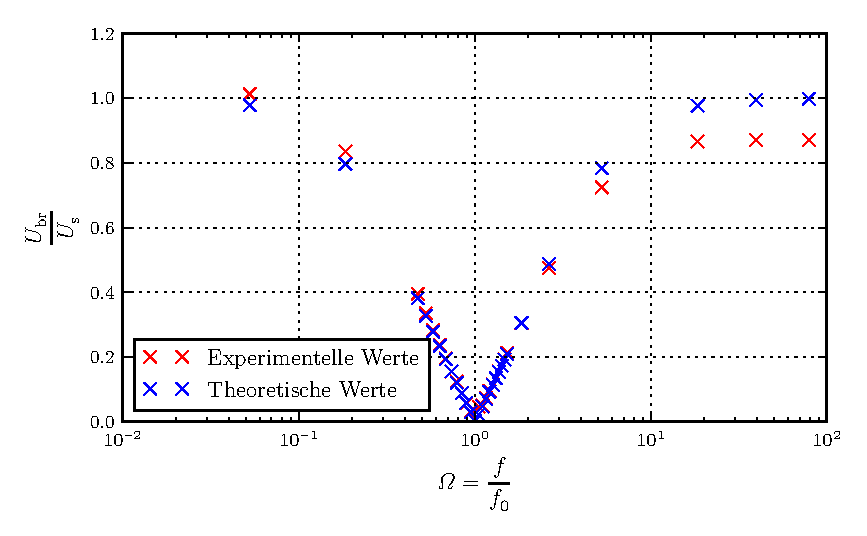
\includegraphics[width=\textwidth]{AufgabeE.pdf}
  \caption{Brückenschaltung}
  \label{fig:AufgabeE}
\end{figure}
